%%%%%%%%%%%%%%%%%%%%%%%%%%%%%%%%%%%%%%%%%
% Short Sectioned Assignment
% LaTeX Template
% Version 1.0 (5/5/12)
%
% This template has been downloaded from:
% http://www.LaTeXTemplates.com
%
% Original author:
% Frits Wenneker (http://www.howtotex.com)
%
% License:
% CC BY-NC-SA 3.0 (http://creativecommons.org/licenses/by-nc-sa/3.0/)
%
%%%%%%%%%%%%%%%%%%%%%%%%%%%%%%%%%%%%%%%%%

%----------------------------------------------------------------------------------------
%	PACKAGES AND OTHER DOCUMENT CONFIGURATIONS
%----------------------------------------------------------------------------------------

\documentclass[paper=a4, fontsize=11pt]{scrartcl} % A4 paper and 11pt font size

\usepackage[T1]{fontenc} % Use 8-bit encoding that has 256 glyphs
\usepackage{palatino} % Use the Adobe Utopia font for the document - comment this line to return to the LaTeX default
\usepackage[english]{babel} % English language/hyphenation
\usepackage{amsmath,amsfonts,amsthm,stmaryrd,amssymb} % Math packages
\usepackage{url}

\usepackage{sectsty} % Allows customizing section commands
\allsectionsfont{\centering \normalfont\scshape} % Make all sections centered, the default font and small caps

\usepackage{fancyhdr} % Custom headers and footers

\usepackage{listings}% http://ctan.org/pkg/listings
\lstset{
	basicstyle=\ttfamily,
	mathescape
}

\usepackage[square]{natbib}
\usepackage{graphicx}

\pagestyle{fancyplain} % Makes all pages in the document conform to the custom headers and footers
\fancyhead{} % No page header - if you want one, create it in the same way as the footers below
\fancyfoot[L]{} % Empty left footer
\fancyfoot[C]{} % Empty center footer
\fancyfoot[R]{\thepage} % Page numbering for right footer
\renewcommand{\headrulewidth}{0pt} % Remove header underlines
\renewcommand{\footrulewidth}{0pt} % Remove footer underlines
\setlength{\headheight}{13.6pt} % Customize the height of the header

\numberwithin{equation}{section} % Number equations within sections (i.e. 1.1, 1.2, 2.1, 2.2 instead of 1, 2, 3, 4)
\numberwithin{figure}{section} % Number figures within sections (i.e. 1.1, 1.2, 2.1, 2.2 instead of 1, 2, 3, 4)
\numberwithin{table}{section} % Number tables within sections (i.e. 1.1, 1.2, 2.1, 2.2 instead of 1, 2, 3, 4)

%\setlength\parindent{0pt} % Removes all indentation from paragraphs - comment this line for an assignment with lots of text

%----------------------------------------------------------------------------------------
%	TITLE SECTION
%----------------------------------------------------------------------------------------

\newcommand{\horrule}[1]{\rule{\linewidth}{#1}} % Create horizontal rule command with 1 argument of height

\title{	
\normalfont \normalsize 
\textsc{University of Stuttgart} \\ [25pt] % Your university, school and/or department name(s)
\horrule{0.5pt} \\[0.4cm] % Thin top horizontal rule
\huge Hauptseminar: Technical Details on the Logjam Attack \\ % The assignment title
\horrule{2pt} \\[0.5cm] % Thick bottom horizontal rule
}

\author{Li Yang Wu} % Your name

\date{\normalsize\today} % Today's date or a custom date

\begin{document}
\pagenumbering{gobble}% Remove page numbers (and reset to 1)
\clearpage
\thispagestyle{empty}
\maketitle % Print the title

\newpage
\tableofcontents

\newpage
\clearpage
\pagenumbering{arabic}% Arabic page numbers (and reset to 1)
%----------------------------------------------------------------------------------------
%	ABSTRACT
%----------------------------------------------------------------------------------------
\section*{Abstract}
\begin{abstract}
In the field of study of security for computer networks, \citep{Adrian:2015:IFS:2810103.2813707} developed a new attack called Logjam to break many cryptographic systems that use Diffie-Hellman key exchange, where TLS 1.2 was the current standard at that time to establish secure end-to-end connections. This work elucidates technical details on the background of Logjam, in particular Diffie-Hellman key exchange, Number Field Sieve algorithm and TLS handshake, and summarizes the overall results.
\end{abstract}
%----------------------------------------------------------------------------------------
%	INTRODUCTION
%----------------------------------------------------------------------------------------
\section{Introduction}
If it comes to network security, Diffie-Hellman key exchange is the standard wildly used in practice and declared to be secure. However, \citep{Adrian:2015:IFS:2810103.2813707} could break the security on many popular and browser certified websites. They demonstrated this so called Logjam attack on the Transfer Level Security protocol that supports Diffe-Hellman as key exchange. They also implemented an attack exploiting the use of small exponents with unsafe primes using a combination of the Pohling-Hellman decomposition and Pollard's lambda method.

Section 2 provides a formal definition of the key exchange problem using asymmetric keys and describes the solution according to \citep{diffie1976new}. In order to break Diffie-Hellman, \citep{gordon1993discrete} first proposed how the Number Field Sieve algorithm can be used to compute logarithms in prime fields. This method is rather complicated and covers a large part of this work in Section 3. While most methods presented here is about cryptography, Section 4 presents the Transport Layer Security, specified in \citep{dierks2008transport}, which is a security protocol used in the transport layer from the OSI model. This model is the most commonly used one that provides a decomposition of a network system into layers, from physical to application level. Section 5 uses the methods from the previous sections to explain Logjam in short. Section 6 presents an attack proposed by \citep{van1996diffie} that exploits a specific kind of bad parameter choices made by system designers when Diffie-Hellman key exchange is used. The second result presented in \citep{Adrian:2015:IFS:2810103.2813707} is an estimate on the cost of computing logs of group elements using 1024 bits primes. I will briefly summarize their assumptions for the estimate and their results in Section 7. A conclusion is drawn about what is necessary to make computer networks more secure in the future in Section 8.
%----------------------------------------------------------------------------------------
%	Diffie-Hellman Key Exchange
%----------------------------------------------------------------------------------------
\section{Diffie-Hellman Key Exchange}
\label{sec:DHKeyExchange}
\citep{diffie1976new} was the first paper presenting a practical solution to the privacy and the authentication problem that does not rely on secure communication channels. These kinds of channels are often not given or so inefficient to use that the benefit of telecommunication is nullified. Hence, it was a historical and great advance in computer networking and cryptography. They presented an asymmetric approach with trap door functions that have an exponential cipher-cryptanalyst ratio. Because of this, a security system can choose feasible large private keys that are at the same time infeasible to infer from public keys and encrypted messages w.r.t. computation time.
\subsection{Problem Formulation}
Given:
\begin{itemize}
	\item $A, B$, the communication partners.
	\item Only insecure communication channels are available.
	\item $\{M\}$, a finite message space which contains all possible messages $M$ to be exchanged.
\end{itemize}
Determine:
\begin{itemize}
	\item $C = (\{E_K\}_{K\in\{K\}}, \{D_K\}_{K\in\{K\}})$, a \textit{public key cryptosystem} with mutual inverse functions
	\begin{itemize}
		\item $E_K:\{M\}\rightarrow\{M\}$
		\item $D_K:\{M\}\rightarrow\{M\}$
	\end{itemize}
	denoted as \textit{encryption} and \textit{decryption transformation} respectively.
	\item $\{K\}$, a suitable set of keys.
	\item Such that
	\begin{enumerate}
	\item $\forall K\in\{K\}:M = D_K(E_K(M))$
	\item $\forall K\in\{K\},M\in\{M\}:E_K(M), D_K(M)$ are easy to compute.
	\item $\forall^\infty K\in\{K\},f:\{E_K\}_{K\in\{K\}}\rightarrow \{D_K\}_{K\in\{K\}}:D_K = f(E_K)$ is infeasible to compute.
	\item $\forall K\in\{K\}\exists g:\{K\}\rightarrow(\{E_K\}_{K\in\{K\}}, \{D_K\}_{K\in\{K\}}):g(K) = (E_K,D_K)$ is feasible to compute.
	\end{enumerate}
\end{itemize}
The goal is therefore to find a key space $\{K\}$ and one transformation generator $g$ to generate public and private keys $(E_K,D_K)$ that fulfil these four conditions above.

The reason we call the public and private keys "encryption" and "decryption" transformations is that these keys can be used for secure message exchange directly. Everyone who wants to send a message $M$ to, say, $A$ just needs to send $E_A(M)$ and $A$ can read $D_A(M)$. This however is slower than cipher algorithms using symmetric keys. For the sake of performance, the solution proposed uses this asymmetric mechanism to exchange a session key, that is then used to encrypt application data.

\subsection{Solutions}
\paragraph{Key Exchange}
The solution the authors propose is to draw public and private keys $(E,D)$ from finite fields $\mathrm{GF}(q)\cong\mathbb{Z}/q\mathbb{Z}$, i.e.
\begin{equation}
E, D \in \mathrm{GF}(q) = \{x \mod q \mid x \in \mathbb{Z}\}.
\end{equation}
By choosing the private key as the logarithm of the public key and an arbitrary basis $\alpha \in \mathrm{GF}(q)$,
\begin{eqnarray}
E = \alpha^D\mod q,\\
D = \log_\alpha E \mod q,\\
1 \leq D,E \leq q-1,
\end{eqnarray}
the requirements 3. and 4. are fulfilled. Calculating $E$ from $D$ has logarithmic time complexity in $q$. Inversely, calculating $D$ from $E$ has a complexity of $\sqrt{q}$. Therefore the cipher-cryptanalyst ratio is exponential. Note that this is not a proven bound. We use the best known algorithms for these problem to get this ratio. Better algorithms have not been found for decades, therefore this method is considered safe. Also, one need to find good primes $q$ in order to assure worst or near worst case log-computation time.

Now if $A$ and $B$ want to exchange a session key, they first choose public and private keys $E_A$, $E_B$, $D_A$, $D_B$ from a number field $\mathrm{GF}(q)$ with a sufficient size $q$ and send each other their public keys over the insecure communication channel. Then, they can calculate the common session key
\begin{eqnarray}
K_{A,B} & = & \alpha^{D_AD_B} \mod q\\
& = & (\alpha^{D_A})^{D_B} \mod q\\
& = & {E_A}^{D_B} \mod q\label{eqn:keyA}\\
& = & (\alpha^{D_B})^{D_A} \mod q\\
& = & {E_B}^{D_A} \mod q.\label{eqn:keyB}
\end{eqnarray}
While $A$ calculates the right term in \ref{eqn:keyA}, $B$ calculates the right term in \ref{eqn:keyB} and both of them now have the same session key $K_{A,B}$.

Because of the trap-door property of this mechanism, it allows us to use it for one-way authentication. A signature $s$ of some user $A$ is $D_A(s)$. No one can forge it, since $D_A$ is private. $A$ cannot deny his or her signature, since everyone can confirm $E_A(D_A(s)) = s$.

\paragraph{Cryptanalysis}
The attacker can compute $K_{A,B}$ either by computing $D_A$ from $E_B$ or $D_B$ from $E_A$, both are log-problems in finite fields. Thus, the attacker is successful iff he or she can afford exponentially more computation power than $A$ and $B$.

%----------------------------------------------------------------------------------------
%	Number Field Sieve Algorithm
%----------------------------------------------------------------------------------------
\section{Number Field Sieve Algorithm}
As described above, the only known way to break Diffie-Hellman is to compute $D$ from $E$, i.e. to compute discrete logs for prime fields for a fixed prime $q$ and base $\alpha$. \citep{gordon1993discrete} first proposed how the \textit{Number Field Sieve} (NFS) algorithm can be used to compute discrete logs. Before that, this technique was known to solve the factorization problem for large primes.

\subsection{Approach}
The idea is to factorize $E$ and find logs for each of these factors. The logs of these factors can be constructed by the logs of some precomputed logs in the database. This step can be done very efficiently. The difficult problem is to build up such a database for the prime of interest $q$. But the good thing is that this precomputation only depends on $q$ and not on a specific problem instance $E$. Once the precomputation is done, the database can be used to compute the log for every $E\in \mathrm{GF}(q)$.

The algorithm for NFS in general is technically difficult to understand. This means that there are many mathematical objects we must deal with and keep in mind at the same time. For simplicity I neglected some details for a better reading, while the drawback is that I cannot show all intermediate steps and instead need to refer to the original paper from time to time.

\subsection{Precomputation}
\label{subsec:precomputation}
The precomputation consists of three steps. In Polynomial Selection, we find an appropriate polynomial representation for $\mathrm{GF}(q)$. Using this representation, we find equations that relate certain numbers with smaller primes in $\mathrm{GF}(q)$ in the Sieving step. These equations form matrices that can be used to find relations that lead to the logs of the base $\alpha$ in the Linear Algebra step. But first, one assumption must be made on $\alpha$.

\subsubsection{Smoothness Assumption}
Define that an integer number $x$ is $B$-smooth, if all prime factors of $x$ are smaller than $B$. NFS assumes the base $\alpha$ to be $B$-smooth where $B$ is an upper bound for the prime values in the factor base (which is the output of the precomputation). $B$ is restricted by our computation capabilities. If $\alpha$ is not $B$-smooth, we can use a $B$-smooth $\alpha'$ instead. Then, we can compute $\log_{\alpha'}\alpha$ and formulate our original problem with
\begin{equation}
\log_\alpha E\equiv\frac{\log_{\alpha'}E}{\log_{\alpha'}\alpha}\mod (q-1)
\text{ .}
\end{equation}
If $\alpha'$ is not a generator for $\mathrm{GF}(q)^*$, the logs on the right hand side might not exist. $\alpha'$ can be checked for feasibility by factoring $(q-1)$ with the NFS factoring algorithm and check
\begin{equation}
(a')^{\frac{q-1}{p}} \not\equiv 1 \mod q,\quad\forall p\parallel q
\text{ ,}
\end{equation}
where $p\parallel q$ denotes that $p$ is a prime divisor of $q$. The reason why $\alpha$ or $\alpha'$ needs to be $B$-Smooth is that the factor base needs to have at least one inhomogeneous relation for the logs of the factor base, using the equation
\begin{eqnarray}
\label{eqn:assumption}
\log_\alpha\alpha = 1 \equiv \sum_{p^t\parallel a}t\log_\alpha p \mod (q-1)
\text{ ,}
\end{eqnarray}
which is not guaranteed to be the case if not all log factors are considered.

\subsubsection{Polynomial Selection}
The goal in the first step is to find a polynomial representation of $\mathrm{GF}(q)$. This has the advantage that we can express relations and encode informations in terms of linear equations to reason about them, which are the tasks that actually will be done in the next steps.

First, we represent $\mathrm{GF}(q)$ as $\mathbb{Z}/q\mathbb{Z}$ where elements are identified with their least non-negative residues. Then, choose an integer $m$ and polynomial $f:\mathbb{Z}\rightarrow\mathbb{Z}$ of degree $k$ such that $f$ is monic, irreducible over $\mathbb{Q}$ and $f(m)\equiv 0 \mod q$. We can find such a polynomial $f$ by choosing $m$ of suitable size and find coefficients $a_1,...,a_k$ such that
\begin{eqnarray}
q = \sum_{i=0}^{k}a_im^i
\text{ .}
\end{eqnarray}
It is required that $q\nmid\Delta_f$, where $\Delta_f$ is the discriminant of $f$. If the choice of $f$ or $m$ leads to $q\mid\Delta_f$, then try another $m$ or alter $f$ slightly, for example add $m$ to $a_i$ and subtract $1$ from $a_{i+1}$.

Next, let $\gamma\in\mathbb{C}$ be the root of $f$, define $K = \mathbb{Q}(\gamma) = \mathbb{Q}\cup\{\gamma\}$ and $O_K$ the ring of integers in $K$. Since $\mathrm{gcd}(q,\Delta_f) = 1$, $\hat{q}:=(q,\gamma-m)$ is a first-degree prime factor of $q\in O_K$. It follows that $O_K/\hat{q}\cong\mathrm{GF}(q)$ and we can define a homomorphism $\phi:\mathbb{Z}[\gamma]\rightarrow\mathbb{Z}/q\mathbb{Z}$, providing us the representation we aimed for. We denote a prime ideal $s\in O_K$ as \textit{good} if $s$ does not divide the index $[O_K:\mathbb{Z}[\gamma]]$, otherwise we denote it as \textit{bad}.

The actual factor base $\mathcal{B}$ for which we want to find the logarithms consists of two parts: $\mathcal{B}_\mathbb{Q}$ the set of rational primes and $\mathcal{B}_K$ the set of good prime ideals in $O_K$, where all of these elements are bounded in size, i.e. $p,\Vert p'\Vert_1\leq B,\ \forall p\in\mathcal{B}_\mathbb{Q},p'\in\mathcal{B}_K$. Note that $B$ is the same bound for our base $\alpha$ (from our primary problem definition: Find $D$ for $E=\alpha^D\mod q$). Also, let $\mathcal{B}'\subset\mathcal{B}_\mathbb{Q}$ denote the set of prime factors of $\alpha$.

\subsubsection{Sieving}
In this step we try to find linear equations that are informative in the sense that they are related to the the logarithms in $\mathcal{B}$. For that, sieve through integer pairs $(c,d)$ that are co-prime for which $c+dm$ and $c+d\gamma$ are $p$-smooth for at least one $p\in\mathcal{B}_\mathbb{Q}$. For this smoothness criteria, we can formulate equations
\begin{eqnarray}
c+dm = \prod_{s\in\mathcal{B}_\mathbb{Q}}s^{w_s(c,d)}
\end{eqnarray}
and
\begin{eqnarray}
|N(c+d\gamma)| = \prod_{s\in\mathcal{B}_\mathbb{Q}}s^{v_s(c,d)}
\text{ ,}
\end{eqnarray}
where $N(c+d\gamma) = (-d)^kf(-\frac{c}{d})$ (see original paper \citep{gordon1993discrete} for explanation), for some $w_s,v_s\in\mathbb{Z}^+$.

From here we can derive factorizations for primes in $\mathcal{B}_K$ with the fact (not proven here) that there is an unique ideal $\hat{s}\in\mathcal{B}_K$ lying over $s$ and dividing $c+d\gamma$. Let $v_{\hat{S}}(c,d) = v_s(c,d)$ for this ideal and be zero for other ideals in $\mathcal{B}_K$ of norm $s$. Then we have the following
\begin{eqnarray}
\label{eqnSieve1}
c+dm = \prod_{s\in\mathcal{B}_\mathbb{Q}}s^{w_s(c,d)}
\end{eqnarray}
and
\begin{eqnarray}
\label{eqnSieve2}
c+d\gamma = \prod_{\hat{s}\in\mathcal{B}_K}\hat{s}^{v_{\hat{s}}(c,d)}
\text{ .}
\end{eqnarray}
Repeat the steps described so far to find more pairs $(c,d)$ to build equations \ref{eqnSieve1} and \ref{eqnSieve2} until we have at least $|\mathcal{B}|$ of these equations. For each equation, build a matrix, where its rows are the $w_s$'s and $v_{\hat{s}}$'s, we call this set $\mathcal{A}$. We modify each $A\in\mathcal{A}$ by extracting only those columns where elements are in $\mathcal{B}-\mathcal{B}'$. This means, we are only interested in solutions for primes $s\in\mathcal{B}'$. $\mathcal{A}$ is now the input for the next step.

\subsubsection{Linear Algebra}
For each $A \in \mathcal{A},\ A = \mathbb{Z}^{S\times T},\ S > T$, where each row has at most $X$ non-zero entries, find a linear relation over $\mathbb{Q}$ for the rows of $A$. This is accomplished in four steps, shown for the case $S=T+1$. This procedure was developed by Carl Pomerance (*1944) which was not separately published, instead only for helping out in \citep{gordon1993discrete}.
\paragraph{Step 1}Attempt to compute the rank $r = \mathrm{rk}(A)$. For that, choose a random prime $q_0\leq XT\log T$. Later, we will check if that choice was feasible. If not, come back here and sample another one. Then, use Gaussian elimination mod $q_0$ to find the rank $r_0$ of $A\mod q_0$. Rearrange the rows so that the first $r_0$ rows are linearly independent mod $q_0$. Now the rearranged matrix is
\begin{equation}
A' =
\begin{pmatrix}
v_1\\v_2\\\vdots\\v_{T\!+\!1}
\end{pmatrix}
=
\begin{pmatrix}
a'_{11} & a'_{12} & \cdots & a'_{1T} \\
a'_{21} & a'_{22} & \cdots & a'_{2T} \\
\vdots & \vdots & \ddots & \vdots \\
a'_{T\!+\!11} & a'_{T\!+\!12} & \cdots & a'_{T\!+\!1T} \\
\end{pmatrix}
\text{ .}
\end{equation}
The result of the Gaussian elimination provides a submatrix $\hat{A} = \mathbb{Z}^{r_0\times r_0}$ of the first $r_0$ rows and columns that is nonsingular mod $q_0$,
\begin{equation}
\hat{A} =
\begin{pmatrix}
v_1\\v_2\\\vdots\\v_{r_0}
\end{pmatrix}
=
\begin{pmatrix}
a'_{11} & a'_{12} & \cdots & a'_{1r_0} \\
a'_{21} & a'_{22} & \cdots & a'_{2r_0} \\
\vdots & \vdots & \ddots & \vdots \\
a'_{r_01} & a'_{r_02} & \cdots & a'_{r_0r_0} \\
\end{pmatrix}
\text{ .}
\end{equation}
\paragraph{Step 2} Attempt to express $v_{r_0+1}$ as a linear combination of $v_1,...,v_{r_0}\mod q$ for each $q\leq XT\log T$. For some $q$ it will be successful, for others not. Denote the product of all successful primes as $\boldsymbol{P}$ and the product of all unsuccessful primes as $\boldsymbol{P'}$. If $\boldsymbol{P'} > XT\log T$, then repeat Step 1 (sample a new random prime number). Otherwise, continue with the next step.
\paragraph{Step 3} Attempt to find the determinant $\mathrm{det}(\hat{A})$ of $\hat{A}$. For each prime $q|\boldsymbol{P}$, use the Wieldemann's probabilistic determinant algorithm \citep{wiedemann1986solving} to compute an integer $D_q\in\{0,...,q-1\}$, which is the determinant of $A\mod q$ with probability of at least $1-(XT)^{-2}$, i.e.
\begin{equation}
\mathbb{P}(D_q = \det(A\mod q)\mid A,q) \geq 1-(XT)^{-2}
\text{ .}
\end{equation}
For each $D_q$ we can write an congruence
\begin{equation}
D_0 \equiv D_q \mod q,\quad\forall q|\boldsymbol{P}
\end{equation}
and use the Chinese remainder theorem to compute $D_0$ fulfilling these congruences and being closest to zero. Repeat this step until we have found a value that lies within the bound
\begin{equation}
0 < |D_0| \leq (X^{\frac{1}{2}}T)^T
\text{ .}
\end{equation}

\paragraph{Step 4} In the final step we try to find the actual coefficients $c_1,...,c_{r_0}$ for the linear relation between $v_{r_0+1}$ and the rest of the rows. Again, use the Chinese remainder theorem to find these coefficients closest to zero such that
\begin{equation}
D_0v_{r_0+1}\equiv\sum_{i=1}^{r_0}c_iv_i\mod\boldsymbol{P}
\text{ .}
\end{equation}
In case one of these coefficients $c_i$ exceeds $(X^{\frac{1}{2}}T)^T$ in absolute value, repeat Step 3 to find another $D_0$. Otherwise, we have found the relation
\begin{equation}
D_0v_{r_0+1}=\sum_{i=1}^{r_0}c_iv_i
\text{ .}
\end{equation}
It can also be shown that the expected runtime of this algorithm is
\begin{equation}
\mathcal{O}(X^2T^3\log^3T)
\text{ .}
\end{equation}

\subsubsection{Results}
Here I sum up the final result not showing details, as it needs more technical preparations that I neglected for simplicity. Feel free to look at the original paper for a complete derivation of the solution.

After applying the algorithm described in the Linear Algebra step on the matrices $\mathcal{A}$ resulted form the Sieving step, we have some new equations
\begin{equation}
\prod_{(c,d)}(c+dm)^{x(c,d)} = U
\textit{ ,}
\end{equation}
where $x(c,d)$ is the solution for the matrix constructed from $(c,d)$ and $U$ is a unit in $O_K$. After some intermediate steps, we can express the logs of primes $s\in\mathcal{B}$ as $z_s$ (which is a black box here) and state
\begin{equation}
\prod_{s\in\mathcal{B}'}s^{z_s}\equiv 1\mod q
\text{ .}
\end{equation}
Taking the log, we have
\begin{equation}
\sum_{s\in\mathcal{B}'}z_s\log_\alpha s \equiv 0 \mod (q-1)
\text{ .}
\end{equation}
With more than $|\mathcal{B}'|$ such congruences, we can solve these with equation \ref{eqn:assumption} and obtain the logs for all primes $s\in\mathcal{B}'$.

\subsection{Individual Log Calculation}
\label{subsec:indiviualLogCalculation}
Now that we have our database ready, we can calculate a private key $D$ given $E$. The first step is to find a sort of a decomposition of $E$ by sampling random integers $l\in{1,..,q-1}$ until we have found an $l$ that satisfies
\begin{equation}
\alpha^lE\equiv p_1p_2\cdots p_t\mod q
\text{ ,}
\end{equation}
where each $p_i$ should be "small", for example $\leq q^\frac{1}{k}$. If the discrete logs $x_i$ of each $q_i$ were known, we could compute $D$ with
\begin{equation}
D = \left(\sum_{i=1}^{t}x_i\right)-l \mod q
\text{ .}
\end{equation}
Finding the log for a certain $p_i$ is a similar procedure as the precomputation, where we computed the logs of factors of $\alpha$. We need to find a suitable polynomial that can be used to express relations between $p_i$ and the factor base $\mathcal{B}'$ in form of linear equations. These equations can also be found by sieving through co-prime pairs $(c,d)$ and cancelling out factors not in $\mathcal{B}'$. This gives us the desired result where $p_i$ can be represented by factors in $\mathcal{B}'$, i.e.
\begin{equation}
p_i \equiv \prod_{s\in\mathcal{B}'}s^{z'_s} \mod q
\end{equation}
and thus
\begin{equation}
\log_{\alpha}p_i = \sum_{s\in\mathcal{B}'}z'_s\log_{\alpha}s \mod (q-1)
\text{ ,}
\end{equation}
where $z'_s$ is some term that comes from intermediate calculation steps that I neglected for simplicity. As described above, the private key $D$ can now be calculated from the $\log_{\alpha}p_i$'s.

Note that improved versions of the NFS algorithm for logarithm calculation exist, such as the one proposed in \citep{joux2003improvements}.
%----------------------------------------------------------------------------------------
%	Transport Layer Security
%----------------------------------------------------------------------------------------
\section{Transport Layer Security}
\label{sec:tls}
The document \citep{dierks2008transport} presents the full Transport Layer Security (TLS) protocol specification. I summarize the handshake section from there because the Logjam attack exploits the protocol flaw exactly here. An abbreviated message flow diagram is shown in Figure \ref{fig:tls}.
\begin{figure*}[h]
	\centering
	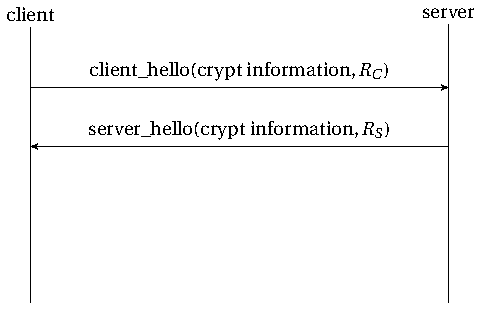
\includegraphics[width=10cm]{../Grafiken/TLS/tls}
	\caption{The message flow diagram of the TLS handshake, abbreviated.}
	\label{fig:tls}
\end{figure*}
\subsection{Hello Messages}
These messages initiate the handshake and exchange information about which cipher methods are supported on each side.
\paragraph{Hello Request} This message is optional and can be sent by the server at any time. The meaning is that the server wishes to renegotiate the connection. It expects to receive the \verb|ClientHello| message next.
\paragraph{Client Hello} With this message, the client wants to establish or re-establish a connection to the server. Several information are sent that are used for negotiation. The \verb|client_version| tells which TLS is used by the client. A random structure that consists of a time stamp and some random bytes are typically used for security checks, for example avoiding replay attacks. The client also offers a list of cipher and compression methods the server can choose from. It can use a session id to reuse security agreements from earlier or other session to abbreviate the handshake.
\paragraph{Server Hello} The server replies symmetrically by sending an \verb|server_version| which is lower or equals the \verb|client_version| and also a random structure that must not depend on the client's random structure. It selects the algorithms for cipher and compression. If none of these algorithms match, the handshake fails. If the client wished to reuse a session, the server sends the same session id back, otherwise it generates a new one.
\paragraph{Server Hello Done}
This message indicates the end of a \verb|ServerHello| message, because its parameters do not have fixed lengths. The client should check all these parameters and also the server's certificate.

\subsection{Certification}
\paragraph{Certificate Request}
The server can request a certificate from the client if this is provided from the security method used. There are specific certificate types for the Diffie-Hellman key exchange method. The client needs to sign its certificate and make sure that the type matches the required one.
\paragraph{Client Certificate}
\begin{sloppypar}
After the client received the \verb|ServerHelloDone| and \verb|RequestCertificate| message from the server, the client sends this message. When there are no suitable certificates available, the content of this message should be empty. Then, the server decides to continue or to deny the handshake.
\end{sloppypar}
\paragraph{Certificate Verification}
When the server receives the certificate from the client, which turns out to be valid, the server sends this message to confirm the acknowledgement.

\subsection{Key Exchange}
TLS supports RSA and DH encryption. After the client has sent its certificate or, if it was necessary, after \verb|ServerHelloDone| was received, the client sends its public key to the server. The procedure for exchanging the session key basically goes according to Section \ref{sec:DHKeyExchange}.

\subsection{Finished}
These messages are the last ones in the handshake phase and the first ones that are encrypted with the newly exchanged session key. One participant sends some encrypted content and the other answers with a proof that it can read the content, thus the handshake was successful. Now application data can be send supposedly secure.

%----------------------------------------------------------------------------------------
%	The Logjam Attack
%----------------------------------------------------------------------------------------
\section{The Logjam Attack}
The previous Sections explained the background for the Logjam attack more in detail than in the original work \citep{Adrian:2015:IFS:2810103.2813707}. Now I summarize the attack in short to show how everything comes together.

For preparation, use NFS precomputation to build log databases for some commonly used 512 bit primes (Section \ref{subsec:precomputation}). When the handshake (Section \ref{sec:tls}) we want to attack begins, catch the \verb|ClientHello| message as man in the middle and rewrite the offered cipher suit such that it only contains all weak ($\leq$ 512 bit) DH methods supported by the server. Since the client expects the server to choose from a strong cipher suit, we need to rewrite the \verb|ServerHello| message and replace the fake cipher suit with one that is strong but methodically matches the fake one. When keys are exchanged (Section \ref{sec:DHKeyExchange}), the client cannot detect any problems because the structure of these messages are the same regardless of which prime field is used. In the last step of the handshake, it is checked via \verb|Finished| messages whether the communication partner knows the secret. The attacker computes the secret (Section \ref{subsec:indiviualLogCalculation}) and replies accordingly. The client now beliefs that the attacker is the server and thereby lost its security.

The success of this attack depends on whether the servers being attacked support number fields of small primes or not. During the experiment it turned out that actually many servers do support those and some of them are even certificated being secure.

%----------------------------------------------------------------------------------------
%	Pohling-Hellman Algorithm
%----------------------------------------------------------------------------------------
\section{Exploiting Use of short Exponents}
Some application designers optimize the computation speed of $\alpha^D$ by choosing small $D$'s. This can be insecure, if the the prime $q$ is not chosen safe, which means that the subgroup generated by $\alpha$ in $\mathrm{GF}(q)$ has small factors. The authors of the Logjam attack also implemented an attack proposed by \citep{van1996diffie} and performed it on servers that have this weakness. This algorithm combines the Pollard's lambda method with the Pohlig-Hellman decomposition. In the following, these two methods are described, before presenting the attack.

\subsection{Pollard lambda} This method is a randomized one that solves a special case of the log problem $E = \alpha^D\mod q$, where the solution $D$ is known to be in range $b<D<b+w$ for some $b,w\in \mathbb{N}$. Using some random function $f:\mathbb{N}\rightarrow R$, with $R\subsetneq\mathbb{N}$ being the range we want to randomize over, ideally tuned to maximize the probability of a success, two sequences of numbers are generated:
\begin{equation}
\begin{array}{lcl}
T & = & (y_0',...,y_N'),\\
W & = & (y_0,...,y_M)
\text{ .}
\end{array}
\end{equation}
Sequence $T$ starts with the value $y_0' = g^{b+w}$ and generates the remaining elements as $y_{i+1}' = y_i'g^{f(y_i')}$. For $W$, $y_0 = E$ and $y_{i+1} = y_ig^{f(y_i)}$. The log distance between $y_0'$ and $y_N'$ that sets both in the following relation
\begin{equation}
\log_\alpha(y_N') = \log_\alpha(y_0') + d_N'
\text{ ,}
\end{equation}
is
\begin{equation}
d_N' = \sum_{i=0}^{N'-1}f(y_i')\mod (q-1)
\text{ .}
\end{equation}
and for $W$ analogously. The $T$ sequence stops at some $N$, while the $W$ sequence stops if there is a hit at some point $M$ such that $y_M = y_N'$ or if $d_M$ exceeds $w+d_N'$. In the first case, the solution
\begin{equation}
D = b + w + d_N' - d_M \mod (q-1)
\end{equation}
is found. Otherwise this iteration failed and we need to restart this procedure.

\subsection{Pohlig-Hellman Decomposition} This method reduces the complexity of the log problem by reducing the size of the problem instance. The idea is to find a good way to infer the original logarithm from smaller logarithms efficiently. Then, the remaining problem is to use existing methods to compute these smaller logarithms. However, the requirement is that the prime power factorization
\begin{equation}
q-1 = \prod_{i=1}^v p_i^{c_i}
\end{equation}
is given. The procedure involves two steps. First, compute $E^{\frac{n}{p_i^{c_i}}},\ i=1..v$. Denote $E':= E^{\frac{n}{p_i^{c_i}}}$ and $\alpha' := \alpha^{\frac{n}{p_i^{c_i}}}$. Because
\begin{equation}
E' = \alpha'^D
\text{ ,}
\end{equation}
the reduced problem definition is now
\begin{equation}
E' = \alpha'^{x_i} \mod (p_i),\quad i=1..v
\text{ .}
\end{equation}
Compute, for example with Pollard lambda method, each $x_i$. With the Chinese remainder theorem we can compute $D$ with the congruences
\begin{equation}
D \equiv x_i \mod p_i
\text{ ,}
\end{equation}
because
\begin{equation}
\prod_{i=1}^v p_i^{c_i} = q-1
\text{ .}
\end{equation}

\subsection{Improved Attack}
Since $q-1$ does not always decompose in a way that every $x_i$ is feasible to compute, we cannot use Pohlig-Hellman to its full extend. But we can still extract some information from those factors $p_i$ that are $B$-smooth, where $B$ is restricted by our computation capabilities. In fact, we can recover $D\mod B_r$ from those $x_i$ that are feasible to compute, where
\begin{equation}
B_r = \prod_{i=1}^r x_i,\quad r\leq v,\ i < i+1
\text{ .}
\end{equation}
If $B_r > D$, the problem is solved. Otherwise we have $k = \log B_r$ bits of information about $D$ that can be used to reduce the computation time of finding $D$.

It can be shown that $k \approx \log B$. Because typically $B < D$ in practice, the expectation is that work is not finished after computing $B_r$. Let $z:=B_r$ and $n:=q-1$, rewrite $n=zQ$, where $Q$ is the product of the remaining factors $q_i$ that are not $B$-smooth. We can compute $V = D \mod z,\ 0\leq V<z$ with a partial Pohlig-Hellman decomposition and represent $D$ in the following way:
\begin{equation}
D = Az + V
\text{ ,}
\end{equation}
where $A$ is now the unknown to be determined. The problem formulation for finding $A$ can be derived as follows:
\begin{equation}
\begin{array}{lcl}
y=g^D=g^{Az+V} & \Rightarrow & A \leq \frac{D}{z}\\
& \Rightarrow & A\in\{0,...,2^c\},\ c\approx u-k\\
& \Rightarrow & \frac{y}{g^V} = g^{Az} = (g^z)^A\\
& \Rightarrow & y^* = h^A,\quad y^* := \frac{y}{g^V}, h := g^z
\text{ .}
\end{array}
\end{equation}
Now we can use Pollard's lambda method to compute $A$, because $A$ is known to lie in a bounded range $\{b,...,b+w\} = \{0,...,2^c\}$, fulfilling the requirement. With $A$ found we also found $D$.

\paragraph{Runtime Complexity} Let $u$ be the number of bits of the binary representation of $D$, i.e. $u = \log D$. Before this method was discovered, the best attack was known to run at $\mathcal{O}(2^{\frac{u}{2}})$ time. This method has an overall cost of $\mathcal{O}(2^{\frac{u}{4}})$, which made key exchange systems that expose these properties even more insecure.

%----------------------------------------------------------------------------------------
%	Security of 1024 bit Groups
%----------------------------------------------------------------------------------------
\section{Security of 1024 bit Groups}
The second part of \citep{Adrian:2015:IFS:2810103.2813707} estimates the cost of attacking DH key exchange with strong 1024 bit groups using NFS, motivated by the leaks from Edward Snowden, a whistle blower and former employee of the \textit{National Security Agency} (NSA). These leaked documents claim that NSA is already breaking cryptographic systems that are considered to be secure.

Based on the most recent records in log computation and factorization at that time, the authors extrapolated a cost of 45 million core-years to do the precomputation for a group using 1024 bit primes and 30 core-days for individual log computation. Assuming specialized hardware to do the job, they estimate a cost of \$8M to buy enough hardware to do the computation in one year just for Sieving and another \$11B to buy multiple Titan supercomputer clusters for the Linear Algebra step. This sum is indeed within the budget that the U.S. government planned for a cryptologic program, where the NSA is part of. Additionally, the leaked documents also contain an architecture of the decrypt infrastructure, which is perfectly consistent with NFS breaking Diffie-Hellman.

If this estimation is correct, then most servers on the world wide web can be attacked successfully by the NSA, as the documents claim.

%----------------------------------------------------------------------------------------
%	DISCUSSION
%----------------------------------------------------------------------------------------
\section{Conclusion}
The inventors of Logjam gave recommendations to system designers on how to improve the security of their systems due to the success of this attack. Software engineers and cryptography experts need to work together more closely to establish a better sensitivity for security overall. Technically, the most secure groups nowadays are elliptic curves. On top of that, it has a much better cipher-cryptanalyst ratio than "$\mathrm{mod}\ q$"-DH or RSA. But it is mathematically hard to understand, which is why it is not wide spread. This obstacle must be overcome as it is really worth the effort. Insecure legacy systems that support weak groups must be replaced by up-to-date ones, which requires to renew security standards at a much higher rate, where collaboration between service providers and browser developers needs to be intensified. This also counteracts state-level threats that have high resource capacities always ready to perform the latest state-of-art attacks at large scales.

%------------------------------------------------

\newpage
\bibliographystyle{apalike}
\bibliography{literature}

\newpage
\pagenumbering{gobble}% Remove page numbers (and reset to 1)
\clearpage
\thispagestyle{empty}
\noindent \textbf{\underline{\smash{Erkl\"{a}rung}}}:\\

\noindent Hiermit erkl\"{a}re ich, dass ich die vorgelegte Arbeit selbstst\"{a}ndig verfasst und keine anderen als die angegebenen Quellen und Hilfsmittel benutzt und die aus fremden Quellen direkt oder indirekt \"{u}bernommenen Gedanken als solche kenntlich gemacht habe.

\noindent Die Arbeit habe ich bisher keiner anderen Stelle zur Bewertung in gleicher oder vergleichbarer Form vorgelegt. Sie wurde bisher nicht ver\"{o}ffentlicht.

\vspace{40pt}
\noindent\begin{tabular}{ll}
	Stuttgart, 21.06.2017 & \\
	\makebox[2.5in]{\hrulefill} & \makebox[2.5in]{\hrulefill}\\
	Ort, Datum & Unterschrift\\[8ex]% adds space between the two sets of signatures
\end{tabular}

\noindent \textbf{\underline{Declaration}}:\\

\noindent I hereby declare that the submitted work is my own unaided work. All direct or indirect sources used are acknowledged as references.

\noindent This work was not previously presented to another examiner in the same or in a comparable version and has not been published.

\vspace{40pt}
\noindent\begin{tabular}{ll}
	Stuttgart, \today & \\
	\makebox[2.5in]{\hrulefill} & \makebox[2.5in]{\hrulefill}\\
	Place, Date & Signature\\[8ex]% adds space between the two sets of signatures
\end{tabular}
\end{document}